\fenicschapter{Finite Element Variational Forms}
              {Finite Element Variational Forms}
              {Robert C. Kirby and Anders Logg}
              {kirby-5}

In Chapter~[kirby-7], we introduced the following canonical
variational problem: Find $u \in V$ such that
\begin{equation} \label{eq:kirby5:canonical}
  a(v, u) = L(v) \quad \forall v \in \hat{V},
\end{equation}
where $\hat{V}$ is a given test space and $V$ is a given trial space.
The bilinear form
\begin{displaymath}
  a: \hat{V} \times V \rightarrow \R
\end{displaymath}
maps a pair of test and trial functions to a real number and is linear
in both arguments. Similarly, the linear form $L: \hat{V} \rightarrow
\R$ maps a given test function to a real number. We also considered
the discretization of nonlinear variational problems: Find $u \in V$
such that
\begin{displaymath}
  F(v; u) = 0 \quad \forall v \in \hat{V}.
\end{displaymath}
Here, $F: \hat{V} \times V \rightarrow \R$ again maps a pair of
functions to a real number. The semilinear form $F$ is linear in the
test function~$v$ but possibly nonlinear in the trial
function~$u$. Alternatively, we may consider the mapping
\begin{displaymath}
  L_u \equiv F(\cdot; u) : \hat{V} \rightarrow \R,
\end{displaymath}
and note that $L_u$ is a linear form on~$\hat{V}$ for any fixed value
of~$u$.

In Chapter~[kirby-7], we also considered the estimation of the error
in a given functional $\mathcal{M} : V \rightarrow \R$. Here, the
possibly nonlinear functional $\mathcal{M}$ maps a given function~$u$
to a real number $\mathcal{M}(u)$.

In all these examples, the central concept is that of a form that maps
a given tuple of functions to a real number. We shall refer to these
as \emph{multilinear forms}. Below, we formalize the concept of a
multilinear form, discuss the discretization of multilinear forms, and
related concepts such as the \emph{action} of a multilinear form.

Much of the FEniCS software is devoted to the formulation of
multilinear forms (UFL), the discretization of multilinear forms
(FIAT, FFC, SyFi) and the assembly of the corresponding discrete
operators (DOLFIN).

%------------------------------------------------------------------------------

\section{Multilinear Forms}

A form is a mapping from the product of a given sequence
$\{V_j\}_{j=1}^{\rho}$ of function spaces to a real number,
\begin{displaymath}
  a : V_1 \times V_2 \times \cdots \times V_{\rho} \rightarrow \R.
\end{displaymath}
If the form~$a$ is linear in each of its arguments, we say that the
form is \emph{multilinear}. The number of arguments~$\rho$ of the form
is the \emph{arity} of the form.

Forms may often be parametrized over one or more
\emph{coefficients}. A typical example is the right-hand side $L$ of
the canonical variational problem~(\ref{eq:kirby5:canonical}), which
is a linear form parametrized over a given coefficient~$f$. We shall
use the notation $a(v; f) \equiv L_f(v) \equiv L(v)$ and refer to the
test function~$v$ as an \emph{argument} and to the function~$f$ as
a \emph{coefficient}. In general, we shall refer to forms which are
linear in each argument (but possibly nonlinear in its coefficients)
as multilinear forms. Such a multilinear form is a mapping from the
product of a sequence of argument spaces $\{V_j\}_{j=1}^{\rho}$ and a
sequence of coefficient spaces $\{W_j\}_{j=1}^n$,
\begin{displaymath}
  \begin{split}
    a &: V_1 \times V_2 \times \cdots \times V_{\rho} \, \times \,
         W_1 \times W_2 \times \cdots \times W_n \rightarrow \R, \\
    a &\mapsto a(v_1, v_2, \ldots, v_{\rho}; w_1, w_2, \ldots, w_n).
  \end{split}
\end{displaymath}
The argument spaces $\{V_j\}_{j=1}^{\rho}$ and coefficient spaces
$\{W_j\}_{j=1}^n$ may all be the same space but they typically differ,
when Dirichlet boundary conditions are imposed on one or more of the
spaces, or when the multilinear form arises from the discretization of
a mixed problem such as in Section~\ref{sec:kirby7:mixed}.

In finite element applications, the arity of a form is typically $\rho
= 2$, in which case the form is said to be bilinear, or $\rho = 1$, in
which case the form is said to be linear. In the special case of $\rho
= 0$, we shall refer to the multilinear form as a
\emph{functional}. It may sometimes also be of interest to consider forms of
higher arity ($\rho > 2$). Below, we give examples of some multilinear
forms of different arity.

\subsection{Examples}

\paragraph{Poisson's equation}

Consider Poisson's equation with variable conductivity~$\kappa =
\kappa(x)$,
\begin{displaymath}
  -\nabla \cdot (\kappa \nabla u) = f.
\end{displaymath}
Assuming Dirichlet boundary conditions on the boundary
$\partial\Omega$ of the domain $\Omega$, the corresponding canonical
variational problem is defined in terms of a pair of multilinear
forms, $a(v, u) = \int_{\Omega} \kappa \nabla v \cdot \nabla u \dx$
and $L(v) = \int_{\Omega} v f \dx$. Here, $a$ is a bilinear form
($\rho = 2$) and $L$ is a linear form ($\rho = 1$). Both forms have
one coefficient ($n = 1$) and the coefficients are $\kappa$ and $f$
respectively:
\begin{displaymath}
  \begin{split}
    a &= a(v, u; \kappa), \\
    L &= L(v; f).
  \end{split}
\end{displaymath}
We usually drop the coefficients from the notation and use the
short-hand notation $a = a(v, u)$ and $L = L(v)$.

\paragraph{The incompressible Navier--Stokes equations}

The incompressible Navier--Stokes equations for the velocity~$u$ and
pressure~$p$ of an incompressible fluid read:
\begin{displaymath}
  \begin{split}
    \dot{u} + \nabla u \cdot u - \nabla \cdot \sigma(u, p) &= f, \\
    \nabla \cdot u &= 0,
  \end{split}
\end{displaymath}
where the stress tensor~$\sigma$ is given by $\sigma(u, p) = 2 \mu
\epsilon(u) - p I$ and $\epsilon$ is the symmetric gradient,
$\epsilon(u) = \frac{1}{2}(\nabla u + (\nabla u)^{\top})$. Consider
here the form obtained by integrating the nonlinear term $\nabla u
\cdot u$ against a test function $v$,
\begin{displaymath}
  a(v; u) = \int_{\Omega} v \cdot \nabla u \cdot u \dx.
\end{displaymath}
This is a linear form ($\rho = 1$) with one coefficient ($n = 1$).  We
may linearize $u = \bar{u} + \delta u$ around a fixed
velocity~$\bar{u}$:
\begin{displaymath}
  a(v; u) = a(v; \bar{u}) + a'(v; \bar{u}) \delta u + \mathcal{O}(\delta u^2).
\end{displaymath}
The linearized operator $a'$ is here given by
\begin{displaymath}
  a'(v, \delta u; \bar{u}) \equiv a'(v; \bar{u}) \delta u = v \cdot
  \nabla \delta u \cdot \bar{u} + v \cdot \nabla \bar{u} \cdot \delta
  u.
\end{displaymath}
This is a bilinear form ($\rho = 2$) with one coefficient ($n = 1)$.
We may also consider the \emph{trilinear} form
\begin{displaymath}
  a(v, u, w) = \int_{\Omega} v \cdot \nabla u \cdot w \dx,
\end{displaymath}
where $w$ may be a given (frozen) value for the convective velocity in
a fixed point iteration for the Navier--Stokes equations. Such a
trilinear form may be assembled into a rank three tensor and applied
to a given vector of expansion coefficients for $w$ to obtain a rank
two tensor (a matrix) corresponding to the bilinear form $a(v, u; w)$.
This is rarely done in practice due to the cost of assembling the
global rank three tensor. However, the corresponding local rank three
tensor may be contracted with the local expansion coefficients for~$w$
on each local cell to compute the matrix corresponding to~$a(v, u;
w)$. We return to this issue below in Chapter~[logg-4].

\paragraph{Lift and drag}

When solving the Navier--Stokes equations, it may be of interest to
compute the lift and drag of some object immersed in the fluid.  The
lift and drag are given by the $z$- and $x$-components of the force
generated on the object (for a flow in the $x$-direction):
\begin{displaymath}
  \begin{split}
    L_{\mathrm{lift}}(;u, p) &= \int_{\Gamma} \sigma(u, p) \cdot \hat{n} \cdot \hat{e}_z \ds, \\
    L_{\mathrm{drag}}(;u, p) &= \int_{\Gamma} \sigma(u, p) \cdot \hat{n} \cdot \hat{e}_x \ds.
  \end{split}
\end{displaymath}
Here, $\Gamma$ is the boundary of the body, $\hat{n}$ is the outward
unit normal of $\Gamma$ and $\hat{e}_x$, $\hat{e}_z$ are unit vectors
in the $x$- and $z$-directions respectively. The arity of both forms
is $\rho = 0$ and both forms have two coefficients.

\begin{figure}
  \begin{center}
    %\psfrag{L}{$z$}
    %\psfrag{D}{$x$}
    %\psfrag{n}{$\hat{n}$}
    %\psfrag{Sn}{$\sigma \cdot \hat{n}$}
    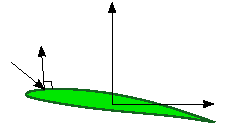
\includegraphics[width=\largefig]{chapters/kirby-5/pdf/lift_drag.pdf}
    \caption{The lift and drag of an object, here a NACA 63A409
      airfoil, are the integrals of the vertical and horizontal
      components respectively of the stress $\sigma \cdot \hat{n}$ over the
      surface~$\Gamma$ of the object. At each point, the product of
      the stress tensor~$\sigma$ and the outward unit normal
      vector~$\hat{n}$ gives the force per unit area acting on the
      surface.}
  \end{center}
\end{figure}

\subsection{Canonical Form}

FEniCS automatically handles the representation and evaluation of a
large class of multilinear forms, but not all. In particular, FEniCS
is currently limited to forms that may be expressed as a sum of
integrals over the cells (the domain), the exterior facets (the
boundary) and the interior facets of a given mesh. In particular,
FEniCS handles forms that may be expressed as the following canonical
form:
\begin{equation} \label{eq:kirby5:integrals}
  a(v_1, v_2, \ldots, v_{\rho}; w_1, w_2, \ldots, w_n)
  =
  \sum_{k=1}^{n_c}   \int_{\Omega_k} I^c_k \dx +
  \sum_{k=1}^{n_f}   \int_{\partial\Omega_k} I^f_k \ds +
  \sum_{k=1}^{n_f^0} \int_{\partial\Omega_k^0} I^{f,0}_k \dS.
\end{equation}
Here, each $\Omega_k$ denotes a union of mesh cells covering a subset
of the computational domain~$\Omega$. Similarly, each $\partial
\Omega_k$ denotes a subset of the facets on the boundary of the mesh
and $\partial \Omega_k^0$ denotes a subset of the interior facets of
the mesh. The latter is of particular interest for the formulation of
discontinuous Galerkin methods that typically involve integrals across
cell boundaries (interior facets).

One may consider extensions of~(\ref{eq:kirby5:integrals}) that
involve point values or integrals over subsets of cells or
facets. Such extensions are currently not supported by FEniCS but may
be added in the future.

\section{Discretizing Multilinear Forms}

As we saw in Chapter~[kirby-7], one may obtain the finite element
approximation $u_h = \sum_{j=1}^N U_j \phi_j \approx u$ of the
canonical variational problem~(\ref{eq:kirby5:canonical}) by solving a
linear system $AU=b$, where
\begin{displaymath}
  \begin{split}
    A_{ij} &= a(\hat{\phi}_i, \phi_j), \quad i,j = 1,2,\ldots,N, \\
    b_i &= L(\hat{\phi}_i), \quad i = 1,2,\ldots,N.
  \end{split}
\end{displaymath}
Here, $A$ and $b$ are the discrete operators corresponding to the
bilinear and linear forms $a$ and $L$ for the given bases of the test
and trial spaces. In general, we may discretize a multilinear form~$a$
of arity~$\rho$ to obtain a tensor~$A$ of rank~$\rho$. The discrete
operator $A$ is defined by
\begin{displaymath}
  A_i = a(\phi^1_{i_1}, \phi^2_{i_2}, \ldots, \phi^{\rho}_{i_{\rho}};
          w_1, w_2, \ldots, w_n),
\end{displaymath}
where $i = (i_1, i_2, \ldots, i_{\rho})$ is a multiindex of
length~$\rho$ and $\{\phi^j_k\}_{k=1}^{N_j}$ is a basis for $V_h^j
\subset V^j$, $j = 1,2,\ldots,\rho$. The discrete operator is a
typically sparse tensor of rank~$\rho$ and dimension $N_1 \times N_2
\times \cdots \times N_{\rho}$.

The discrete operator~$A$ may be computed efficiently using an
algorithm known as~\emph{assembly}, which is the topic of the next
chapter. As we shall see then, an important tool is the \emph{cell
  tensor} obtained as the discretization of the bilinear form on a
local cell of the mesh. In particular, consider the discretization of
a multilinear form that may be expressed as a sum of local
contributions from each cell~$K$ of a mesh~$\mathcal{T} = \{K\}$,
\begin{displaymath}
  a(v_1, v_2, \ldots, v_{\rho}; w_1, w_2, \ldots, w_n)
  = \sum_{K\in\mathcal{T}} a_K(v_1, v_2, \ldots, v_{\rho}; w_1, w_2, \ldots, w_n).
\end{displaymath}
This corresponds to the case $n_c = 1$, $n_f = n_f^0 = 0$ and $\Omega_1
= \Omega$ in~(\ref{eq:kirby5:integrals}). Discretizing~$a_K$ using the
local finite element basis~$\{\phi^{K,j}_j\}_{j=1}^{n_j}$ on~$K$, we
obtain the cell tensor
\begin{equation} \label{eq:kirby5:celltensor}
  A^K_i
  = a_K(\phi^{K,1}_{i_1}, \phi^{K,2}_{i_2}, \ldots, \phi^{K,\rho}_{i_{\rho}}; w_1, w_2, \ldots, w_n).
\end{equation}
The cell tensor~$A^K$ is a typically dense tensor of rank~$\rho$ and
dimension $n_1 \times n_2 \times \cdots \times n_{\rho}$. The discrete
operator $A$ may be obtained by appropriately summing the
contributions from each cell tensor $A^K$. We return to this in detail
below in Chapter~[logg-3]. Below, we will sometimes refer to $A^K$ the
element tensor.

\begin{figure}
  \begin{center}
    %\psfrag{K}{$K$}
    %\psfrag{S}{$S$}
    %\psfrag{AK}{$A^K=$}
    %\psfrag{AS}{$A^S=$}
    %\psfrag{AS0}{$A^{S,0}=$}
    %\psfrag{A}{$A=$}
    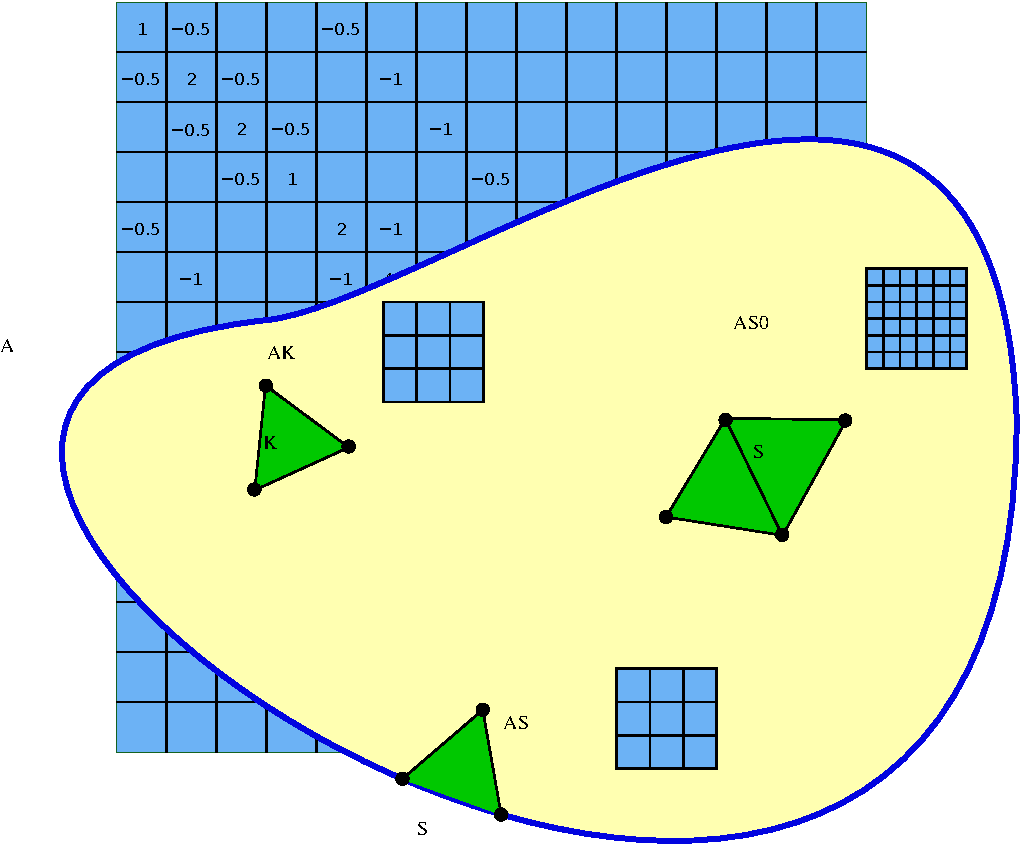
\includegraphics[width=\largefig]{chapters/kirby-5/pdf/element_tensors.pdf}
    \caption{The cell tensor~$A^K$, exterior facet tensor $A^S$ and
      interior facet tensor $A^{S,0}$ on a mesh are obtained by
      discretizing the local contribution to a multilinear form on a
      cell, exterior facet or interior facet
      respectively.}
    \label{fig:kirby5:tensors}
  \end{center}
\end{figure}

If $\Omega_k \subset \Omega$, the discrete operator $A$ may be
obtained by summing the contributions only from the cells covered by
$\Omega_k$. One may similarly define the exterior and interior facet
tensors $A^S$ and $A^{S,0}$ as the contributions from a facet on the
boundary or the interior of the mesh. The exterior facet tensor $A^S$
is defined as in~(\ref{eq:kirby5:celltensor}) by replacing the domain
of integration $K$ by a facet $S$. The dimension of $A^S$ is generally
the same as that of $A^K$. The interior facet tensor $A^{S,0}$ is
defined slightly differently by considering the basis on a \emph{macro
  element} consisting of the two elements sharing the common facet~$S$
as depicted in Figure~\ref{fig:kirby5:tensors}. For details, we refer
to~\cite{OlgaardLoggWells2008}.

\section{The Action of a Multilinear Form}

Consider the bilinear form
\begin{displaymath}
  a(v, u) = \int_{\Omega} \nabla v \cdot \nabla u \dx,
\end{displaymath}
obtained from the discretization of the left-hand side of Poisson's
equation. Here, $v$ and $u$ are a pair of test and trial functions.
Alternatively, we may consider~$v$ to be a test function and $u$ to be
a given solution to obtain a \emph{linear} form parametrized over the
coefficient~$u$,
\begin{displaymath}
  (\mathcal{A} a) (v) \equiv a(v; u) = \int_{\Omega} \nabla v \cdot \nabla u \dx.
\end{displaymath}
We refer to the linear form $\mathcal{A}a$ as the \emph{action} of the
bilinear form~$a$. In general, the action of a $\rho$-linear form with
$n$ coefficients is a $(\rho-1)$-linear form with $n+1$ coefficients.
In particular, the action of a bilinear form is a linear form, and the
action of a linear form is a functional.

The action of a bilinear form plays an important role in the
definition of matrix-free methods for solving differential
equations. Consider the solution of a variational problem of the
canonical form~(\ref{eq:kirby5:canonical}) by an Krylov subspace
method such as GMRES (Generalized Minimal RESidual
method)~\cite{SaadSchultz1986} or CG (Conjugate Gradient
method)~\cite{HestenesStiefel1952}. Krylov methods approximate the
solution $U\in\R^N$ of the linear system $AU=b$ by finding an
approximation for $U$ in the subspace of $\R^N$ spanned by the vectors
$b, Ab, A^2b, \ldots, A^kb$ for some $k \ll N$. These vectors may be
computed by repeated application of the discrete operator $A$ defined
as above by
\begin{displaymath}
  A_{ij} = a(\phi^1_i, \phi^2_j).
\end{displaymath}
For any given vector $U \in \R^N$, it follows that
\begin{displaymath}
  (A U)_i = \sum_{j=1}^N A_{ij} U_j
  = \sum_{j=1}^N a(\phi^1_i, \phi^2_j) U_j
  = a\left(\phi^1_i, \sum_{j=1}^N U_j \phi^2_j\right)
  = a(\phi^1_i; u_h),
\end{displaymath}
where $u_h = \sum_{j=1}^N U_j \phi^2_j$ is the finite element
approximation corresponding to the coefficient vector~$U$.
In other words, the application of the matrix~$A$ on a given
vector~$U$ is given by the action of the bilinear form evaluated
at the corresponding finite element approximation,
\begin{displaymath}
  (A U)_i = (\mathcal{A} a) (\phi^2_i; u_h).
\end{displaymath}
The variational problem $(\ref{eq:kirby5:canonical})$ may thus be
solved by repeated evaluation (assembly) of a linear form (the action
$\mathcal{A} a$ of the bilinear form~$a$) as an alternative to first
computing (assembling) the matrix~$A$ and then repeatedly computing
matrix--vector products with~$A$. Which approach is more efficient
depends on how efficiently the action may be computed compared to
matrix assembly, as well as on available preconditioners. For a
further discussion on the action of multilinear forms, we refer
to~\cite{BagheriScott2004}.

\section{The Derivative of a Multilinear Form}

When discretizing nonlinear variational problems, it may be of
interest to compute the derivative of a multilinear form with respect
to one or more of its coefficients. Consider the nonlinear variational
problem to find $u \in V$ such that
\begin{equation} \label{eq:kirby5:nonlinear}
  F(v; u) = 0 \quad \forall v \in V.
\end{equation}
To solve this problem by Newton's method, we linearize $u = \bar{u} +
\delta u$ around a fixed value~$\bar{u}$ to
obtain
\begin{displaymath}
  0 = F(v; u) \approx F(v; \bar{u}) + F'(v; \bar{u}) \delta u.
\end{displaymath}
Given an approximate solution $\bar{u}$ of the nonlinear variational
problem~(\ref{eq:kirby5:nonlinear}), we may then hope to improve the
approximation by solving the linear variational problem
\begin{displaymath}
  F'(v, \delta u; \bar{u}) \equiv F'(v, \bar{u}) \delta u = -F(v; \bar{u}).
\end{displaymath}
Here, $F'$ is a bilinear form with two arguments $v$ and $\delta u$,
and one coefficient $\bar{u}$, and $-F$ is a linear form with one
argument $v$ and one coefficient $\bar{u}$.

When there is more than one coefficient, we will use the notation
$\mathcal{D}_w$ to denote the derivative with respect to a specific
coefficient~$w$. In general, the derivative $\mathcal{D}$ of a
$\rho$-linear form with $n > 0$ coefficients is a $(\rho+1)$-linear
form with $n$ coefficients. To solve the variational
problem~(\ref{eq:kirby5:nonlinear}) using a matrix-free Newton method,
we would thus need to repeatedly evaluate the linear form
$(\mathcal{A}\mathcal{D}_u F) (v; \bar{u}_h, \delta u_h)$ for a given
finite element approximation~$\bar{u}_h$ and increment $\delta u_h$.

Note that one may equivalently consider the application of Newton's
method to the nonlinear discrete system of equations obtained by a
direct application of the finite element method to the variational
problem~(\ref{eq:kirby5:nonlinear}) as discussed in Chapter~[kirby7].

\section{The Adjoint of a Bilinear Form}

The adjoint $a^*$ of a bilinear form~$a$ is the form obtained by
interchanging the two arguments,
\begin{displaymath}
  a^*(w, v) = a(v, w) \quad \forall v \in V^1 \quad \forall w \in V^2.
\end{displaymath}
The adjoint of a bilinear form plays an important role in the error
analysis of finite element methods as we saw in~Chapter~[kirby-7] and
as will be discussed further in Chapter~[massing] where we consider
the linearized adjoint problem (the dual problem) of the general
nonlinear variational problem~(\ref{eq:kirby5:nonlinear}). The dual
problem takes the form
\begin{displaymath}
  (\mathcal{D}_u F)^* (v, z; u) = \mathcal{D}_u M (v; u) \quad \forall v \in V,
\end{displaymath}
or simply
\begin{displaymath}
  F'^* (v, z) = M' (v) \quad \forall v \in V,
\end{displaymath}
where $(\mathcal{D}_u F)^*$ is a bilinear form and $\mathcal{D}_u
\mathcal{M}$ is a linear form (the derivative of the
functional~$\mathcal{M}$).

\section{A Note on the Order of Test and Trial Functions}

It is common in the literature to consider bilinear forms where the
trial function~$u$ is the first argument, and the test function~$v$ is
the second argument,
\begin{displaymath}
  a = a(u, v).
\end{displaymath}
With this notation, one is lead to define the discrete operator~$A$ as
\begin{displaymath}
  A_{ij} = a(\phi^2_j, \phi^1_i).
\end{displaymath}
In this book and throughout the code and documentation of the FEniCS
Project, we have instead adopted the notation
\begin{displaymath}
  a = a(v, u),
\end{displaymath}
which leads to the more natural definition
\begin{displaymath}
  A_{ij} = a(\phi^1_{i}, \phi^2_j),
\end{displaymath}
which is particularly convenient when we consider multilinear forms of
general arity. This ordering follows naturally from the ordering of
dimensions for a matrix (rows before columns) and agrees with the fact
that the rows of a matrix correspond to equations (test functions) and
the columns to unknowns (expansion coefficients for the trial
functions).
